Figures \ref{fig:undelayed_measurement}-\ref{fig:delayed_measurement} depict the normal situation where measurements are available without delay and the situation of interest herein where the availability of measurements involves a delay.

When there is a delay between the time at which a sensor takes a measurement 
and the time that it is available for the the state estimation measurement update, the estimation procedure must address this delay.
To do otherwise (i.e., ignore the delay) can significantly affect performance.
Similarly if a measurements is corrupted by an uncertain bias, it needs to be mitigated in the estimation process.
This article describes an approach to address the delay and bias in the measurement for a discrete-time state-space model.
\todo{AN: Comment out this note after you read this.

Following are some recommended practices for good writing that I corrected in the draft.
\begin{enumerate}
	\item Do not start a sentence with a symbol.
	\item All figures and tables must be referred to by a label/name and discussed in the text.
	\item Use a consistent format for referring to figures. The call in column 2 page 2 i not consistent. 
	\item If a figure is not created by you, but copied from somewhere else, you must cite the source. 
	\item Insert adequate spacing in equations so that separate symbols are easy to detect. Search `$\,$' to find my fixes.
\end{enumerate}
I am noting them, because if I just fixed them, then you would not know for the future.}

\begin{figure}[b]
	%trim={Left Bottom Right Top}
	% \fbox%
	{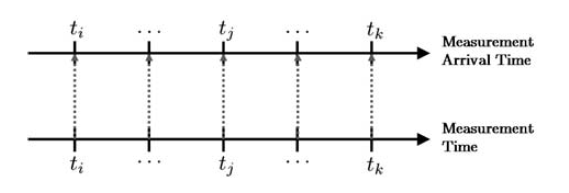
\includegraphics[width=1.0\columnwidth]{./img/undelayed_measurement.png}}
	\caption{Sequence of measurements unaffected by delay. \red Source ???}
	\label{fig:undelayed_measurement}
\end{figure} 

\begin{figure}[b]
	%trim={Left Bottom Right Top}
	% \fbox%
	{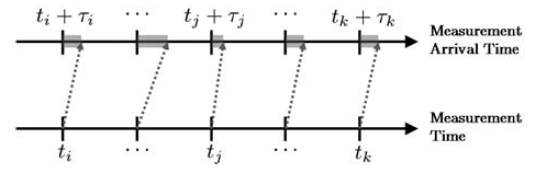
\includegraphics[width=1.0\columnwidth]{./img/delayed_measurement.png}}
	\caption{Sequence of measurements affected by delay. \red Source ???}
	\label{fig:delayed_measurement}
\end{figure} 


 